\documentclass[10 pt]{article}
\usepackage{tikz}
\usetikzlibrary{arrows}
\usepackage[margin=0.5 in]{geometry}
\usepackage[utf8]{inputenc}
\usepackage{tabu}
\usepackage{color}
\usepackage{xcolor}
\usepackage{listings}
\usepackage{enumitem}
\usepackage{siunitx}
\usepackage{multicol}
\usepackage{titlesec} 

\setlength{\columnsep}{1cm} 
\titleformat{\subsection}[runin]
{\normalfont\large\bfseries}{\thesubsection}{1em}{}
\titleformat{\subsubsection}[runin]
{\normalfont\normalsize\bfseries}{\thesubsubsection}{1em}{}

\title{\textbf {Estructuras de Datos 1 - ST0245\\Examen Parcial 2 - Jueves (033)
}}
\author{Nombre ..............................\\
		Departamento de Informática y Sistemas\\
		Universidad EAFIT\\}
\date{Octubre 24 de 2019}
\begin{document}
\lstdefinestyle{customc}{
	language=Java, 
	numbers=left, 
	showspaces=false,
    showstringspaces=false, 
    tabsize=2, 
    breaklines=true,
    xleftmargin=5.0ex,
}
\lstset{escapechar=@,style=customc, numbers=left, stepnumber = 1} 
\maketitle

\textbf{En las preguntas de selección múltiple, una respuesta incorrecta tendrá
una deducción de 0.2 puntos en la nota final. Si dejas la pregunta sin
responder, la nota será de 0.0. Si no conoces la respuesta, no adivines.}


\begin{multicols}{2}
\section{1. Tablas de Hash 20\%}
En los videojuegos, las tablas de hash se usan para guardar la información de las armas; por ejemplo,
su ataque, su velocidad y su duración. Considera la siguiente función de hash para cadenas de caracteres.
La constante \texttt{TABLE\_SIZE} representa el tamaño máximo del arreglo con el que se representa 
internamente la tabla de hash.

{\footnotesize
\begin{lstlisting}
private int funcionHash(String k){
  return ((int) k.charAt(0)) % TABLE_SIZE;
}
\end{lstlisting}
}
\begin{enumerate}[label=\alph*]
	\item (10\%) ¿Qué problema presenta esa función hash? Las cadenas...
	{\small
	\begin{enumerate}[label=\roman*]
		% Respuesta: Todas las cadenas que inician con la misma letra colisionan
		\item  que terminan con la misma letra colisionan
		\item  que inician con la misma letra colisionan
		\item  cuya suma de los caracteres es la misma colisionan
		\item  que tienen los mismos caracteres colisionan
	\end{enumerate}
	}
	\item (10\%) ¿Cuál es la complejidad asintótica, en el peor de los casos, de \texttt{funcionHash(k)}? Donde $n$ es la longitud de la cadena $k$.
	\begin{enumerate}[label=\roman*]
		% Respuesta: $O(1)$
		\item $O(n)$
		\item $O(n^2)$
		\item $O(n\log n)$
		\item $O(1)$
	\end{enumerate}
\end{enumerate}


\section{2. Listas 20\%}
Liko escribió un nuevo método para una lista simplemente enlazada. Desafortunamente, Liko olvidó
qué hace el método. ¿Podrías ayudarnos a decifrar qué retorna el método \texttt{mistery} y su complejidad?
{\footnotesize
\begin{lstlisting}
class Node { 
   int val; 
   Node next; 
   Node(int d) { val = d; } 
} 
class Algorithms { 
  static Node mistery(Node l1, Node l2) {
    Node temp = new Node(0);
    Node p=temp;
    Node p1=l1;
    Node p2=l2;
    while(p1!=null && p2!=null){
        if(p1.val < p2.val){
            p.next = p1;
            p1 = p1.next;
        }else{
            p.next = p2;
            p2 = p2.next;  }
        p=p.next;              }
    if(p1!=null){
        p.next = p1;    }
    if(p2!=null){
        p.next = p2;    }
    return temp.next;
 }
}
\end{lstlisting}
}
\begin{enumerate}[label=\alph*]
	\item (10\%) ¿Qué retorna el algoritmo anterior?
	\begin{enumerate}[label=\roman*]
		% Respuesta: una nueva lista con los elementos de ambas listas ordenados
		\item Una nueva lista donde \texttt{l2} está al final de \texttt{l1}
		\item Suponiendo que \texttt{l1} y \texttt{l2} están ordenadas, una nueva lista con los elementos de ambas listas ordenados
		\item Una nueva lista donde \texttt{l2} está al final de \texttt{l1}
		\item La lista \texttt{l1}
	\end{enumerate}
	\item (10\%) ¿Cuál es la complejidad asintótica, en el peor de los casos, del algoritmo anterior? Donde $n$ es la longitud de la lista que inicia en el nodo \texttt{l1} y $m$ es la longitud de la lista que inicia en el nodo \texttt{l2}
	\begin{enumerate}[label=\roman*]
		% Respuesta: $O(n+m)$
		\item $O(n \times m)$
		\item $O(n + m)$
		\item $O(n\log m)$
		\item $O(m \times (\log n)^2)$
	\end{enumerate}
\end{enumerate}



\section{3. Grafos  20\%}
Considera el siguiente grafo no dirigido:
\begin{center}
		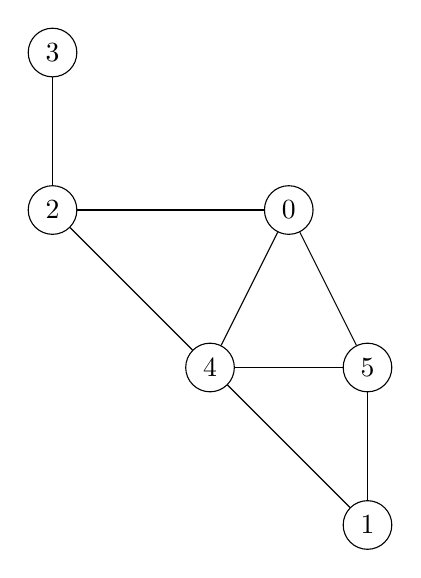
\begin{tikzpicture}
		
		\tikzset{vertex/.style = {shape=circle,draw,minimum size=1.5em}}
		\tikzset{edge/.style = {-,> = latex'}}
		\node[vertex] (0) at (0,0)  {0};
		\node[vertex] (5) at (1,-2)  {5};
		\node[vertex] (4) at (-1,-2)  {4};
		\node[vertex] (1) at (1,-4)  {1};
		\node[vertex] (2) at (-3, 0) {2};
		\node[vertex] (3) at (-3, 2) {3};
		%edges
		\draw[edge] (0) to (4);	
		\draw[edge] (0) to (5);
		\draw[edge] (5) to (4);
		\draw[edge] (5) to (1);
		\draw[edge] (4) to (1);
		\draw[edge] (4) to (2);
		\draw[edge] (0) to (2);
		\draw[edge] (2) to (3);
		\end{tikzpicture}
	\end{center}
	\begin{enumerate}[label=\alph*)]
		\item (10\%) ¿Cuál es un recorrido de \emph{búsqueda primero en profundidad} del grafo anterior, si como nodo inicial se toma el nodo 1?
		\begin{enumerate}[label=\roman*)]
			\item 1, 5, 0, 3, 2, 4
			\item 1, 4, 5, 0, 2, 3
			\item 1, 4, 0, 3, 5, 2
			\item 1, 5, 4, 0, 3, 2
		\end{enumerate}
	    \item (10\%) ¿Cuál es un recorrido de \emph{búsqueda primero en amplitud} del grafo anterior, si se toma como nodo inicial el nodo 1?
	    \begin{enumerate}[label=\roman*)]
	    	\item 1, 4, 5, 0, 2, 3
	    	\item 1, 5, 0, 2, 3, 4
	    	\item 1, 4, 2, 0, 3, 5
	    	\item 1, 3, 0, 4, 5, 2
	    \end{enumerate}
	\end{enumerate}

\section{4. Árboles binarios de búsqueda 20\%}
Considera el siguiente árbol:
\begin{center}
	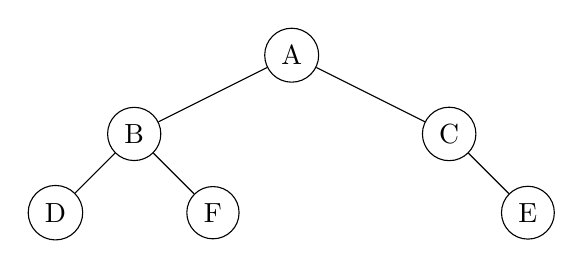
\begin{tikzpicture}
	\tikzset{vertex/.style = {shape=circle,draw,minimum size=1.5em}}
	\tikzset{edge/.style = {-,> = latex'}}
	\node[vertex] (0) at (0,0)  {A};
	\node[vertex] (1) at (-2,-1)  {B};
	\node[vertex] (2) at (2, -1) {C};
	\node[vertex] (3) at (-3, -2) {D};
	\node[vertex] (4) at (3, -2) {E};
	\node[vertex] (5) at (-1, -2) {F};
	%edges
	\draw[edge] (0) to (1);
	\draw[edge] (0) to (2);
	\draw[edge] (1) to (3);
	\draw[edge] (1) to (5);
	\draw[edge] (2) to (4);
	\end{tikzpicture}
\end{center}
\begin{enumerate}[label=\alph*]
	\item (10\%) ¿Qué configuración de vértices $[A, B, C, D, E, F]$ hacen el árbol anterior un árbol de búsqueda binaria?
	\begin{enumerate}[label=\roman*]
		% Respuesta: iv) $[8, 6, 9, 4, 7, 10]$
		\item $[5, 7, 1, 4, 9, 8]$
		\item $[-1, 4, 9, 8, 6, 5]$
		\item $[11, 4, 7, 9, 3, 1]$
		\item $[8, 6, 9, 4, 7, 10]$
	\end{enumerate}
	\item (10\%) ¿Cuál es la complejidad asintótica, en el peor de los casos, de encontrar un elemento en un árbol de búsqueda binaria que se autobalancea como, por ejemplo, el árbol rojo negro o el árbol AVL?
	\begin{enumerate}[label=\roman*]
		% Respuesta: i) $O(log n)$
		\item $O(n)$
		\item $O(1)$
		\item $O(\log n)$
		\item $O(n \log n)$
	\end{enumerate}
	
\end{enumerate}

\section{5. Pilas 20\%}
Dijkstra escribió un algoritmo para convertir una \emph{expresión matemática infija} en 
\emph{notación polaca inversa}, pero se le borraron algunas líneas y no había hecho \emph{commit} en git. La notación polaca inversa evita el uso de
paréntesis; para lograrlo primero se colocan los operandos y luego 
los operadores. Considera los siguientes ejemplos:
{\small
\begin{itemize}
  \item \texttt{postfix(``( 5 + 7 ) * 2'')} retorna \texttt{``5 7 + 2 *''}
  \item \texttt{postfix(``5 + 7 / 2'')} retorna \texttt{``5 7 2 / +''}
\end{itemize}
}



%https://eddmann.com/posts/shunting-yard-implementation-in-java/
{\footnotesize
\begin{lstlisting}
String postfix(String infix) {
 String ops = "+-*/";
 StringBuilder output = new StringBuilder();
 Deque<String> stack  = new LinkedList<>();
 for (String token : infix.split(" ")) {
  if (ops.contains(token)){//es un operador
     while ( ! stack.isEmpty() && isHigherPrec(token, stack.peek()))
       output.append(stack.pop()).append(' ');
     stack.push(token);  
  } else if (token.equals("(")) { // es un (
     stack.push(token);
  } else if (token.equals(")")) { // es un )
     while ( ! stack.peek().equals("("))
       output.append(stack.pop()).append(' ');
     stack.pop();
  } else {   // es un digito
     output.append(...........).append(' ');
  }
 }
 while ( ! stack.isEmpty())
    output.append(stack.pop()).append(' ');
 return output.toString();
}
\end{lstlisting}
}

\begin{enumerate}[label=\alph*]
	\item (10\%) Completa, por favor, la línea 21\\
	% Respuesta:  token
	$\rule{8cm}{0.15mm}$


	\item (10\%) ¿Cuál es la complejidad asintótica, en el peor de los casos, de la operación \texttt{pop()} de una pila?
	\begin{enumerate}[label=\roman*]
		% Respuesta: $O(1)$
		\item $O(n^2)$
		\item $O(n)$
		\item $O(1)$
		\item $O(n^2 \times \log n)$
	\end{enumerate}
\end{enumerate}

{\small
La clase \texttt{StringBuilder} es una implemención de cadenas de caracteres 
con listas enlazadas. La clase \texttt{Deque} es una implementación de una
pila con listas enlazadas. El método \texttt{isHigherPrec(a,b)} retorna verdadero
si $a$ tiene mayor precedencia que $b$; de lo contrario, falso. El método \texttt{S.append(B)} agrega
los caracteres de un \texttt{String} $B$ al final del \texttt{StringBuilder} $S$. El método \texttt{peek()}
permite ver el elemento en el tope de una pila sin retirarlo. El método \texttt{pop()} retira un elemento
de una pila y lo retorna. El método \texttt{push(e)} ingresa el elemento $e$ a una pila. El método \texttt{S.split(`` '')}
genera un arreglo de cadenas separando la cadena $S$ por espacios. El ciclo \texttt{for(String token : infix.split(" "))} se lee como ``para cada \texttt{String token} en el arreglo \texttt{infix.split(" ")}, de izquierda a derecha, haga...'' El método \texttt{A.contains(b)} retorna verdadero si $b$ está en A; de lo contrario, falso.
}

% String postfix(String infix)
% {
%         String ops = "+-*/";
%         StringBuilder output = new StringBuilder();
%         Deque<String> stack  = new LinkedList<>();

%         for (String token : infix.split("\\s")) {
%             // operator
%             if (ops.contains(token)) {
%                 while ( ! stack.isEmpty() && isHigherPrec(token, stack.peek()))
%                     output.append(stack.pop()).append(' ');
%                 stack.push(token);

%             // left parenthesis
%             } else if (token.equals("(")) {
%                 stack.push(token);

%             // right parenthesis
%             } else if (token.equals(")")) {
%                 while ( ! stack.peek().equals("("))
%                     output.append(stack.pop()).append(' ');
%                 stack.pop();

%             // digit
%             } else {
%                 output.append(token).append(' ');
%             }
%         }

%         while ( ! stack.isEmpty())
%             output.append(stack.pop()).append(' ');

%         return output.toString();
% }



\end{multicols}
\end{document}